\documentclass[12pt,a4paper]{article}

\usepackage[utf8]{inputenc}
\setlength{\parindent}{0pt}
\emergencystretch=2em
\usepackage{amsmath,amssymb}
\usepackage[margin=2.3cm]{geometry}
\usepackage{xcolor}
\usepackage[most]{tcolorbox}
\usepackage{tabularx, array}
\usepackage{enumitem}
\usepackage{booktabs}
\usepackage{longtable}
\usepackage{fancyhdr}
\usepackage[hidelinks]{hyperref}
\usepackage{titlesec}
\usepackage{float}

\setlength{\parskip}{4pt}
\setlist{itemsep=1pt,topsep=3pt}
\setcounter{secnumdepth}{3}
\setcounter{tocdepth}{2}

\definecolor{azulprin}{RGB}{0,45,114}
\definecolor{rojoprin}{RGB}{190,0,20}

\titleformat{\section}{\Large\bfseries\color{azulprin}}{\thesection.}{0.6em}{}[\color{azulprin}\titlerule]
\titleformat{\subsection}{\large\bfseries\color{azulprin}}{\thesubsection}{0.6em}{}
\titleformat{\subsubsection}{\normalsize\bfseries\color{rojoprin}}{\thesubsubsection}{0.6em}{}

\pagestyle{fancy}
\fancyhf{}
\fancyhead[L]{\small Procesos de Manufactura}
\fancyhead[R]{\small Formulario -- Semanas 1 a 5}
\fancyfoot[C]{\thepage}
\renewcommand{\headrulewidth}{0.4pt}

% ---------- cajas ----------
\newtcolorbox{defi}[1][]{enhanced,breakable,colback=blue!4,colframe=azulprin,
  fonttitle=\bfseries\small,title={#1},boxrule=0.6pt,arc=2pt,left=6pt,right=6pt,top=3pt,bottom=3pt}
\newtcolorbox{formu}[1][]{enhanced,breakable,colback=yellow!12,colframe=orange!80!black,
  fonttitle=\bfseries\small,title={#1},boxrule=0.6pt,arc=2pt,left=6pt,right=6pt,top=3pt,bottom=3pt}
\newtcolorbox{aviso}[1][]{enhanced,breakable,colback=red!5,colframe=rojoprin,
  fonttitle=\bfseries\small,title={#1},boxrule=0.6pt,arc=2pt,left=6pt,right=6pt,top=3pt,bottom=3pt}
\newtcolorbox{compl}[1][]{enhanced,breakable,colback=green!5,colframe=green!40!black,
  fonttitle=\bfseries\small,title={#1},boxrule=0.6pt,arc=2pt,left=6pt,right=6pt,top=3pt,bottom=3pt}

\newcommand{\ud}[1]{\,\mathrm{#1}}

\begin{document}
\thispagestyle{fancy}

% =====================================================================
\section{Dimensiones}
% =====================================================================

Convención: \textbf{minúsculas para ejes}, \textbf{MAYÚSCULAS para agujeros}.

\begin{center}
	\small
	\begin{tabularx}{\linewidth}{lllX}
		\toprule
		\textbf{Concepto}   & \textbf{Eje} & \textbf{Agujero} &
		\textbf{Significado}
		\\
		\midrule
		Dimensión nominal   & $d_N$        & $D_N$            & Valor
		teórico respecto al que se consideran las medidas límites
		\\
		Dimensión efectiva  & $d_e$        & $D_e$            & Valor
		real, medido sobre la pieza ya construida
		\\
		Dimensión máxima    & $d_M$        & $D_M$            & Valor
		extremo superior de la dimensión
		efectiva
		\\
		Dimensión mínima    & $d_m$        & $D_m$            & Valor
		extremo inferior de la dimensión
		efectiva
		\\
		Diferencia superior & $d_s$        & $D_s$            & Dim.\
		máxima $-$ nominal
		\\
		Diferencia inferior & $d_i$        & $D_i$            & Dim.\
		mínima $-$ nominal                                            \\
		Tolerancia          & $t$          & $T$              &
		Variación máxima permitida de la medida
		\\
		\bottomrule
	\end{tabularx}
\end{center}

\begin{figure}[h!]
	\centering
	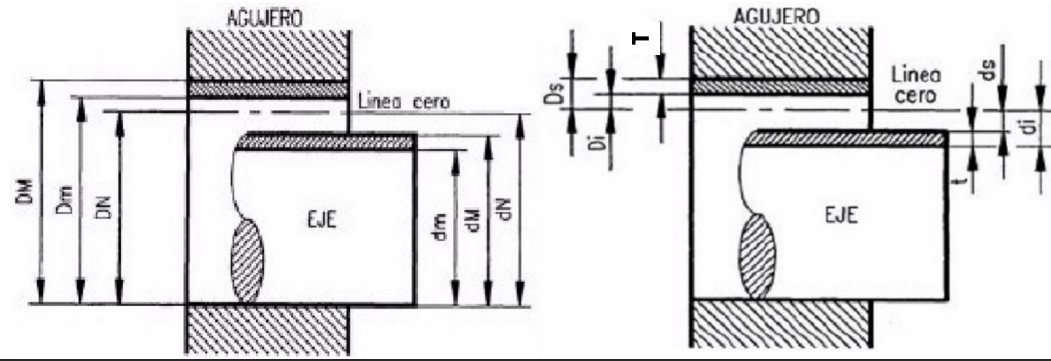
\includegraphics[width=\linewidth]{img/dimensiones.png}
\end{figure}

\begin{formu}[Relaciones fundamentales]
	\centering
	\begin{tabular}{@{}p{7cm}p{7cm}@{}}
		\textbf{Agujeros}           & \textbf{Ejes}               \\[2pt]
		$D_s = D_i + T$             & $d_s = d_i + t$             \\[2pt]
		$D_M = D_m + T$             & $d_M = d_m + t$             \\[2pt]
		$T = D_M - D_m = D_s - D_i$ & $t = d_M - d_m = d_s - d_i$ \\[2pt]
		$D_M = D_N + D_s$           & $d_M = d_N + d_s$           \\[2pt]
		$D_m = D_N + D_i$           & $d_m = d_N + d_i$           \\
	\end{tabular}
\end{formu}

% =====================================================================
\section{Ajustes}
% =====================================================================

\begin{formu}[Ajuste móvil o con juego]
	$J = D_e - d_e > 0$\\
	$J_M = D_M - d_m$ (juego máximo)\\
	$J_m = D_m - d_M$ (juego mínimo)\\
	$T_J = J_M - J_m = T + t$ (tolerancia del juego)
\end{formu}

\begin{formu}[Ajuste fijo o con aprieto]
	$A = d_e - D_e > 0$\\
	$A_M = d_M - D_m$ (aprieto máximo)\\
	$A_m = d_m - D_M$ (aprieto mínimo)\\
	$T_A = A_M - A_m = T + t$ (tolerancia del aprieto)
\end{formu}

\begin{formu}[Ajuste indeterminado]
	$I = D_e - d_e < 0 \;\text{ ó } > 0$\\
	$J_M = D_M - d_m$ \qquad $A_M = d_M - D_m$\\
	$T_I = J_M + A_M = T + t$ (tolerancia del ajuste indeterminado)
\end{formu}

% =====================================================================
\section{Parámetros del torneado}
% =====================================================================

\begin{formu}[1. Velocidad de corte]
	\[ v = n\left(\frac{D_i}{2}\right) \]
	$v$ = velocidad de corte (m/min); $n$ = velocidad de giro o angular del chuck
	(rev/min = rpm), con 1 rev $= 2\pi$; $D_i$ = diámetro inicial (m).\\
	En la práctica: $v = \dfrac{\pi\, D_i\, n}{1000}$ con $D_i$ en mm y $v$ en
	m/min
	(el factor $2\pi$ convierte revoluciones a radianes y el 1000 pasa mm a m).
\end{formu}

\begin{formu}[2. Velocidad lineal (de avance)]
	\[ v_L = n\cdot a \]
	$v_L$ = velocidad lineal o de avance; $n$ = rpm; $a$ = avance (mm/rev). Con
	$a$
	en mm/rev el resultado queda en mm/min.
\end{formu}

\begin{formu}[3. Caudal de viruta]
	\[ Q = v_L \cdot A \qquad (Q = V/t) \]
	$V$ = volumen, $t$ = tiempo, $v_L$ = velocidad lineal o de avance, $A$ = área
	de la sección de material removido (área de la corona circular en cilindrado:
	$A
		= \tfrac{\pi}{4}(D_i^2 - D_f^2)$).
\end{formu}

\begin{formu}[4. Profundidad de corte o de pasada]
	\[ p_T = \frac{D_i - D_f}{2} \qquad\qquad p_T = N_D P_D + N_A P_A \]
	$p_T$ = profundidad total; $N_A$, $N_D$ = número de pasadas de acabado ($N_A =
		0$ si no se especifica) y de
	desbaste; $P_D$, $P_A$ = profundidad de desbaste y de acabado. \textbf{El
		número
		de pasadas debe ser entero.}\\
	Rangos: \textbf{acabado} $P_A \approx 0.1$--$0.5$ mm;
	\textbf{desbaste} $P_D \approx 0.4$--$3$ mm.\\
\end{formu}

\begin{formu}[5. Tiempo de pasada]
	\[ t_p = \frac{L + y + \Delta}{v_L} = \frac{L + y + \Delta}{a\cdot n} \]
	$L$ = longitud a mecanizar; $y$ = retiro de cuchilla (1--3 mm); $\Delta$ =
	distancia por efecto del ángulo de posición $\omega$, con $\tan\omega =
		p/\Delta$, $p$ = profundidad de pasada.\\
	Si $\omega = 45^\circ \Rightarrow \Delta = p$; si $\omega = 90^\circ
		\Rightarrow \Delta = 0$.
\end{formu}

\begin{formu}[6. Tiempo de maquinado]
	\[ t_m = N\left(\frac{L + y + \Delta}{a\cdot n}\right) \]
	$N$ = número de pasadas. Si hay desbaste y acabado con parámetros distintos,
	se suman los tiempos de cada etapa: $t_m = t_D + t_A$.
\end{formu}


% =====================================================================
\section{Parámetros de fresado}
% =====================================================================

\begin{formu}[Parámetros básicos]
	\textbf{Velocidad de corte (m/min):}
	\[ V_c = \frac{\pi\, D\, N}{1000} \]
	$D$ = diámetro de la fresa (mm); $N$ = velocidad de rotación (rpm).
	(Despejando:
	$N = \dfrac{1000\,V_c}{\pi D}$.)\\[4pt]
	\textbf{Profundidades de pasada:} radial $a_e$ y axial $a_p$ (mm).\\[4pt]
	\textbf{Velocidad de avance:} $V_f$ (mm/min).\\[4pt]
	\textbf{Avance por filo (mm/filo):}
	\[ f_z = \frac{V_f}{N\, z} \qquad\left(V_f = f_z\, N\, z\right) \]
	$z$ = número de filos de la fresa.
\end{formu}

\begin{formu}[Espesor de viruta]
	El espesor de viruta $a_c$ \textbf{varía a lo largo del recorrido del diente};
	depende de la posición angular $\psi$ del diente.\\[3pt]
	Si $\kappa_r = 90^\circ$: $\quad a_c = f_z \sin\psi \quad$ y el máximo es
	$a_{c,max} = f_z$.\\[3pt]
	Si $\kappa_r \neq 90^\circ$: $\quad a_c = f_z \sin\psi\,\sin\kappa_r$.
\end{formu}

\begin{formu}[Sección de viruta]
	Sección de material arrancada por un diente = espesor de corte $\times$
	anchura de corte:
	\[ S_c = a_c \cdot a_w \]
	Como el espesor varía en cada instante, \textbf{la sección de viruta también
		varía}.
\end{formu}

\begin{formu}[Fuerza de corte]
	\[ F_c = p_s \cdot S_c \]
	$p_s$ = presión (energía) específica de corte. Al igual que en torneado
	depende del material y de los parámetros de corte. \textbf{En fresado es
		variable por dos motivos:} $S_c$ es variable y $p_s$ es función de $a_c$,
	que
	también varía. Se descompone en fuerza \textbf{axial} $F_a$, \textbf{radial}
	$F_r$ y de corte $F_c$. La fuerza varía periódicamente en el tiempo (golpes de
	cada diente) y puede cambiar de signo.\\
	La curva $p_s(a_c)$ muestra la zona habitual de fresado (espesores de viruta
	pequeños) frente a la de torneado (espesores mayores).
\end{formu}

\begin{formu}[Potencia de corte]
	Como $F_c$ es variable con el tiempo y puede haber varios dientes en corte a
	la vez, no es posible un cálculo simple:
	\[ P_c = F_c(t)\, V_c = S_c(t)\, p_s(a_c)\, V_c = a_c(t)\, a_w\, p_s(a_c(t))\,
		V_c \quad \text{(¡cálculo complicado!)} \]
	Por eso se calcula un \textbf{valor medio} con el valor medio de la energía
	específica de corte $p_s^*$ (se obtiene de tablas a partir del espesor medio
	de
	corte $\bar a_c$) multiplicado por el volumen de viruta mecanizado por unidad
	de
	tiempo:
	\[ P_m = p_s^*(\bar a_c)\, V_f\, a_p\, a_e \qquad\quad \bar a_c =
		\frac{1}{\Theta}\int_0^{\Theta} a_c\, d\theta = \frac{2\, a_e\, f_z\,
			\sin\kappa_r}{\Theta\, D} \]
	Nótese que $V_f\, a_p\, a_e$ es el \textbf{caudal de viruta} $Q$ (volumen
	removido por unidad de tiempo), de modo que $P = p_s\cdot Q$.
\end{formu}

% =====================================================================
\section{Parámetros del taladro}
% =====================================================================

\begin{formu}[Parámetros básicos]
	\textbf{Velocidad de corte (m/min):}
	\[ V_c = \frac{\pi\, D\, N}{1000} \qquad\Longleftrightarrow\qquad N =
		\frac{1000\,V_c}{\pi D} \]
	$D$ = diámetro de la broca (mm); $N$ = velocidad de rotación (rpm).\\[4pt]
	\textbf{Velocidad de avance (mm/min):} $V_f$.\\[4pt]
	\textbf{Avance por filo (mm/diente):}
	\[ f_z = \frac{V_f}{z\, N} \]
	$z$ = número de filos. Con $f = z\,f_z$ (avance por vuelta, mm/rev): $\;V_f =
		f\cdot N$.
\end{formu}

\begin{formu}[Espesor, anchura y sección de viruta]
	\[ a_c = f_z \sin\kappa_r \qquad a_w = \frac{D/2}{\sin\kappa_r} \qquad S_c =
		a_c\, a_w \;\;\text{o también}\;\; S_c = f_z\,\frac{D}{2} \]
	$a_c$ = espesor de corte (mm); $a_w$ = anchura de viruta (mm); $S_c$ = sección
	de viruta (mm$^2$); $\kappa_r$ = ángulo de posición del filo principal. Para
	una broca de 2 filos, $f_z = f/2$.
\end{formu}

\begin{formu}[Fuerza y potencia de corte]
	\[ F_c = p_s\, S_c \qquad\qquad P_c = \frac{z\cdot F_c\cdot \dfrac{V_c}{2}}{60}
		\;\;\text{(W)} \]
	$F_c$ (N); $p_s$ = energía (presión) específica de corte (N/mm$^2$); $V_c$
	(m/min). El factor $V_c/2$ aparece porque la velocidad de corte varía de 0 en
	el
	centro a $V_c$ en el borde; se toma el valor medio (a mitad del radio). El 60
	pasa de m/min a m/s.
\end{formu}

\begin{compl}[Complemento: fórmulas usadas en los ejercicios (no están en la
		teoría)]
	\begin{itemize}[nosep]
		\item \textbf{Altura de la punta:} $h = \dfrac{D}{2\tan(\alpha_p/2)} =
			      \dfrac{D}{2\tan 59^\circ}$ con $\alpha_p = 118^\circ$.
		\item \textbf{Longitud de penetración:} $L = e + h + s$, con $e$ = espesor
		      (profundidad) del agujero, $h$ = altura de la punta y $s$ = salida de
		      seguridad
		      (si es agujero pasante). Equivale a $h=\dfrac{D}{2}\tan(90^\circ -
			      \alpha_p/2) =
			      \dfrac{D}{2}\tan 31^\circ$.
		\item \textbf{Tiempo de corte:} $t_c = \dfrac{L}{V_f} = \dfrac{L}{f\,N}$.
		\item \textbf{Potencia y par:} $P = \dfrac{2\pi N T}{60}$ (W, con $T$ en
		      N$\cdot$m y $N$ en rpm), de donde $T = \dfrac{60\,P}{2\pi N}$.
		\item \textbf{Potencia en el husillo:} $P_h = \eta\, P_{motor}$.
		\item \textbf{Potencia de corte:} $P_c = F_c\, v_c$ (con $v_c$ en m/s); con
		      pérdidas: $P_{total} = P_c(1 + \text{pérdidas})$ (como lo hace la
		      diapositiva).
		\item \textbf{Caudal de viruta (tasa de remoción):} $\dot z = \dfrac{\pi
				      D^2}{4}\, f\, N$; y $P = E_s\,\dot z$ con $E_s$ la energía
		      específica de corte
		      (J/m$^3$).
		\item \textbf{Taladrado con picado (\emph{peck drilling}):} número de
		      penetraciones $n = \dfrac{\text{profundidad}}{\text{penetración por
					      ciclo}}$.
		\item \textbf{Producción:} $Q = \dfrac{3600}{t_{total}}$ agujeros/hora (con
		      $t_{total}$ en s, incluyendo tiempos muertos).
	\end{itemize}
\end{compl}

\end{document}
